% !TeX root = main.tex

%\setkeys{Gin}{draft}

%\singlespacing
%\onehalfspacing

\section{Lab Assignment Goals}
\vspace{.25cm}
\justifying
\par The objective of this lab was to investigate the behavior of a differential pair of MOS composed of $Q_1$ and $Q_2$, and to analyze the distinctions between single-ended and differential signaling, with particular emphasis on their effect on the common mode rejection ratio (CMRR). The circuit was implemented using the ALD1105 MOSFET array. Differential operation was examined to evaluate its effectiveness in enhancing noise rejection and improving signal integrity. LTSpice simulations were utilized to validate theoretical predictions. In addition, worst-case and Monte Carlo analyses were performed to assess variability and robustness.

\begin{center}
\begin{figure}[H]
\includegraphics[scale=0.5]{Chapter_6/Lab_06_Image_1.png}
\caption{Pin-out and block diagram of the ALD1105. \textbf{Note: The body of the NMOS devices ($V^{-}$) was connected to the source, and the body of the PMOS devices ($V^{+}$) was connected to its source.}}
\label{Ch6_fig:1}
\end{figure}
\end{center}

\section{Experiment 1: MOS Differential Pair}

The MOS differential pair circuit, shown in Figure \ref{Ch6_fig:1}, was constructed with the Analog Discovery Studio. The following tasks were completed:

\begin{itemize}
    \item Resistances $R_{D}$ and $R_{CS}$ were measured and recorded in the summary table.
    \item The DC operating point was determined by measuring the node voltages and calculating the drain currents. The results were documented in the summary table.
\end{itemize}

\begin{itemize}
    \item{One of the most common questions asked is the difference between single-ended and differential signal inputs, and what applications they should be considered in.}
    \cite{dwyeromega2025}
\end{itemize}

\begin{center}
\begin{circuitikz}[american,scale=0.8]
\ctikzset{tripoles/mos style=arrows}
\draw
(-3,0) node[nmos,scale=2] (Q1) {}
(3,0) node[nmos,scale=2,xscale=-1] (Q2) {}
(Q1.center) node[right] {$Q_{1}$}
(Q2.center) node[left] {$Q_{2}$}
(Q1.S) -- (Q2.S)
(Q1.D) to[R=$R_{D}$] ++(0,3) node[vdd] {$+V_{DD}$}
(Q2.D) to[R=$R_{D}$] ++(0,3) node[vdd] {$+V_{DD}$}
(Q1.G) to[short,-o] ++(-0.5,0) node[left] {$v_{I1}$}
(Q2.G) to[short,-o] ++(0.5,0) node[right] {$v_{I2}$}
(Q1.S) to[open] ++(3,0) to[R=$R_{CS}$,*-] ++(0,-3) node[vss] {$-V_{SS}$}
(Q1.D) to[short,*-o] ++(-1,0) node[left] {$V_{X}$}
(Q1.D) to[short,-o] ++(1,0) node[right] {$-$}
(Q2.D) to[short,*-o] ++(1,0) node[right] {$V_{Y}$}
(Q2.D) to[short,-o] ++(-1,0) node[left] {$+$} to[open] ++(-1.55,0) node[left] {$v_{o}$}
;
\end{circuitikz}
\vspace{.5cm}
\par
Circuit Parameters: $V_{DD} = 12$ V, $-V_{SS} = -12$ V, $R_{D} = 18$k $\Omega$, $R_{CS} = 10$k $\Omega$, $V_{I1} = V_{I2} = 0$ V
\vspace{.5cm}
\emph{MOS Differential Pair Circuit}
\label{Ch6_fig:3}
\end{center}

\section{Experiment 2: AC Response}
\justifying{
The AC response of the differential pair was evaluated by determining the differential gain, the common-mode gain, and calculating the common-mode rejection ratio (CMRR). Measurements were performed for single-ended output (at node $V_{Y}$ with respect to the ground) and differential output (measuring voltage across nodes $V_{Y}$ and $V_{X}$). The following procedures were followed:}

\begin{itemize}
    \item For the differential input, a sinusoidal signal was applied to the positive input terminal and an equal but opposite phase signal was applied to the negative terminal, while both function generators were synchronized and biased appropriately.
    \item For common-mode input, identical sinusoidal signals were applied to both input terminals without phase offset. 
    \item Both wave generators were synchronized and appropriately biased.
    \item During AC analysis in LTSpice, the measured resistor values were used.
    \item The results were documented in the summary tables that have been provided on the following pages.
\end{itemize}

\begin{center}
	\begin{table}[H]
		\renewcommand{\arraystretch}{0.95}
		\begin{tabular}{ | >{\centering\arraybackslash} m{2.5cm} | >{\centering\arraybackslash} m{2.5cm} |  >{\centering\arraybackslash} m{2.5cm} |}
			\hline
			Quantity & Measured & Units \\ \hline
			$R_{D}$ & 18.025 & k$\Omega$ \\ \hline
			$R_{D}$ & 17.975 & k$\Omega$ \\ \hline
			$R_{CS}$ & 9.839 & k$\Omega$ \\ \hline
		\end{tabular}
	\caption{Resistor Summary}	
	\end{table}
\end {center}

\begin{table}[H]
\renewcommand{\arraystretch}{0.95}
\begin{tabular}{ | >{\centering\arraybackslash} m{2.5cm} | >{\centering\arraybackslash} m{2.5cm} |  >{\centering\arraybackslash} m{2.5cm} | >{\centering\arraybackslash} m{2.5cm} | >{\centering\arraybackslash} m{2.5cm} |}
\hline
\multicolumn{5}{|c|}{DC Operating Point}        \\ \hline
Device & Quantity & Simulated  & Measured & Units \\ \hline
\multirow{5}{*}{$Q_{1}$} & $I_{D}$  & 562.943 & 483.141 & $\mu$A   \\ \cline{2-5} 
                  & $|V_{OV}|$ & 1.407 & 1.141 & V \\ \cline{2-5} 
                  &  $V_{G}$ & 0.000 & 0.000 & V  \\ \cline{2-5} 
                  & $V_{D}$ & 3.063 & 2.896 & V \\ \cline{2-5} 
                  & $V_{S}$ & -1.891 & -1.820 & V \\ \hline
\multirow{5}{*}{$Q_{2}$} & $I_{D}$  & 558.043 & 524.011 & $\mu$A   \\ \cline{2-5} 
                  & $|V_{OV}|$ & 1.407 & 1.140 & V \\ \cline{2-5} 
                  &  $V_{G}$ & 0.000 & 0.000 & V  \\ \cline{2-5} 
                  & $V_{D}$ & 2.060 & 2.011 & V \\ \cline{2-5} 
                  & $V_{S}$ & -1.700 & -1.819 & V \\ \hline
\end{tabular}
\end{table}

\section{Background}
\justifying
In contrast to single-ended signaling, where the signal is measured with respect to a fixed potential (usually ground), differential signaling uses two complementary signals referenced to a common-mode voltage. 
\cite{razaviDifferentialPair}
This configuration provides several advantages:
\begin{itemize}
    \item \textbf{Immunity to environmental noise}: External interference affects both lines equally, and the differential measurement cancels out this noise.
    \item \textbf{Rejection of power supply noise}: Voltage fluctuations in the supply appear as common-mode noise, which is rejected by the differential pair.
    \item \textbf{Reduction of coupled noise}: Crosstalk and interference from adjacent signal lines are minimized.
\end{itemize}
\cite{palermoLab6}


\newpage

\begin{center}
	\renewcommand{\arraystretch}{1.2}
	\begin{table}[H]
	\begin{tabular}{ | >{\centering\arraybackslash} m{3.5cm} |  >{\centering\arraybackslash} m{3cm} | >{\centering\arraybackslash} m{3cm} | >{\centering\arraybackslash} m{2cm} |}
	\hline
	\multicolumn{4}{|c|}{AC Summary - Single Ended}        \\ \hline
	Quantity & Simulated  & Measured & Units \\ \hline
	$A_{d}$  & 6.018 & 6.205 & V/V   \\ \cline{1-4} 
	$A_{d}$ & 15.580 & 15.801 & dB \\ \cline{1-4} \hline
	 &  &  &  \\ \hline
	$A_{cm}$  & 0.840 & 0.499 & V/V   \\ \cline{1-4}
	$A_{cm}$ & -1.515 & -5.924 & dB \\ \cline{1-4} \hline
	 &  &  &  \\ \hline
	CMRR  & 17.104 & 21.724 & dB   \\ \cline{1-4}
\end{tabular}
\caption{AC Summary Table - Single Ended Output}
\end{table}

\end{center}

\begin{center}
\renewcommand{\arraystretch}{1.2}
\begin{table}[H]
\begin{tabular}{ | >{\centering\arraybackslash} m{3.5cm} |  >{\centering\arraybackslash} m{3cm} | >{\centering\arraybackslash} m{3cm} | >{\centering\arraybackslash} m{2cm} |}
\hline
\multicolumn{4}{|c|}{AC Summary - Differential}        \\ \hline
Quantity & Simulated  & Measured & Units \\ \hline
$A_{d}$  & 12.020 & 12.024 & V/V   \\ \cline{1-4} 
$A_{d}$ & 21.598 & 21.578 & dB \\ \cline{1-4} \hline
 &  &  &  \\ \hline
$A_{cm}$  & 0.001 & 0.053 & V/V   \\ \cline{1-4}
$A_{cm}$ & -61.379 & -26.760 & dB \\ \cline{1-4} \hline
 &  &  &  \\ \hline
CMRR  & 59.872 & 48.328 & dB   \\ \cline{1-4}
\end{tabular}
\caption{AC Summary Table - Differential Output}
\end{table}
\end{center}

%\newpage
\textbf{\textcolor{black}{Calculations and Methodology:}}
\vspace{0.3cm}

\noindent
\[
V_P = V_{in1} - V_{GS1} = V_{in2} - V_{GS2}
\]
\[
V_{in1} - V_{in2} = V_{GS1} - V_{GS2}
\]

% \textbf{\textcolor{black}{Equation (1):}}
\begin{tcolorbox}[colback=white,colframe=black,title=]
\begin{equation}
V_{in1} - V_{in2} = V_{GS1} - V_{GS2}
\end{equation}
\end{tcolorbox}

\vspace{0.5cm}

\noindent
\textbf{\textcolor{black}{Assuming $M_1$ and $M_2$ in saturation:}}
\[
(V_{GS} - V_{TH})^2 = \frac{2 I_D}{\mu_n C_{ox} \frac{W}{L}}
\]

% \textbf{\textcolor{black}{Equation (2):}}
\begin{tcolorbox}[colback=white,colframe=black,title=]
\begin{equation}
{V_GS} = \sqrt{\frac{2 I_D}{\mu_n C_{ox} \frac{W}{L}}} + {V_TH}
\end{equation}
\end{tcolorbox}

\begin{tikzpicture}[remember picture, overlay]
\node at (13.8,4.3) {\textcircled{2}};
\end{tikzpicture}

\vspace{0.5cm}

\noindent
\textbf{\textcolor{black}{From Eq. 1 \& 2:}}
\[
V_{in1} - V_{in2} = \sqrt{\frac{2 I_{D1}}{\mu_n C_{ox} \frac{W}{L}}} 
- \sqrt{\frac{2 I_{D2}}{\mu_n C_{ox} \frac{W}{L}}}
\]

\vspace{0.5cm}

\noindent
\textbf{\textcolor{black}{Squaring both sides, and since:}} \quad $I_{SS} = I_{D1} + I_{D2}$

\begin{tcolorbox}[colback=white,colframe=black,title=]
\begin{equation}
{(V_{in1} - V_{in2})^2 = \frac{2}{\mu_n C_{ox} \frac{W}{L}} \left (I_{SS} - 2 \sqrt{I_{D1} I_{D2}} \right)}
\end{equation}
\end{tcolorbox}

\vspace{0.5cm}

\noindent
% \textbf{\textcolor{blue}{Previous equation can be written:}}
\begin{equation}
\frac{\mu_n C_{ox}}{2} \frac{W}{L} (V_{in1} - V_{in2})^2 - I_{SS} = -2 \sqrt{I_{D1} I_{D2}}
\end{equation}

\vspace{0.25cm}

\noindent
% \textbf{\textcolor{blue}{Squaring the two sides, and since:}}
\begin{equation}
4 I_{D1} I_{D2} = (I_{D1} + I_{D2})^2 - (I_{D1} - I_{D2})^2 = I_{SS}^2 - (I_{D1} - I_{D2})^2
\end{equation}

\vspace{0.25cm}

\noindent
% \textbf{\textcolor{blue}{We arrive at:}}
\begin{equation}
(I_{D1} - I_{D2})^2 = -\frac{1}{4} \left( \frac{\mu_n C_{ox}}{W/L} \right)^2 (V_{in1} - V_{in2})^4 
+ I_{SS} \frac{\mu_n C_{ox}}{W/L} (V_{in1} - V_{in2})^2
\end{equation}

\vspace{0.25cm}

% \begin{tcolorbox}[colback=white,colframe=black,title=]
\begin{equation}
I_{D1} - I_{D2} = \frac{\mu_n C_{ox}}{2} \frac{W}{L}(V_{in1} - V_{in2}) 
\sqrt{\frac{4 I_{SS}}{\mu_n C_{ox} \frac{W}{L}} - (V_{in1} - V_{in2})^2}
\end{equation}
% \end{tcolorbox}

\vspace{0.25cm}

\noindent
% \textbf{\textcolor{blue}{Previous equation can be written:}}
\begin{equation}
\frac{\mu_n C_{ox}}{2} \frac{W}{L} (V_{in1} - V_{in2})^2 - I_{SS} = -2 \sqrt{I_{D1} I_{D2}}
\end{equation}

\vspace{0.25cm}

\noindent
% \textbf{\textcolor{blue}{Squaring the two sides, and since:}}
\begin{equation}
4 I_{D1} I_{D2} = (I_{D1} + I_{D2})^2 - (I_{D1} - I_{D2})^2 = I_{SS}^2 - (I_{D1} - I_{D2})^2
\end{equation}

\vspace{0.25cm}

\noindent
% \textbf{\textcolor{blue}{We arrive at:}}
\begin{equation}
(I_{D1} - I_{D2})^2 = -\frac{1}{4} \left( \frac{\mu_n C_{ox}}{W/L} \right)^2 (V_{in1} - V_{in2})^4 
+ I_{SS} \frac{\mu_n C_{ox}}{W/L} (V_{in1} - V_{in2})^2
\end{equation}

\vspace{0.25cm}

\begin{tcolorbox}[colback=white,colframe=black,title=]
\begin{equation}
I_{D1} - I_{D2} = \frac{\mu_n C_{ox}}{2} \frac{W}{L}(V_{in1} - V_{in2}) 
\sqrt{\frac{4 I_{SS}}{\mu_n C_{ox} \frac{W}{L}} - (V_{in1} - V_{in2})^2}
\end{equation}
\end{tcolorbox}

\vspace{0.25cm}

\noindent
\begin{center}
Let \quad $\Delta V_{in} = V_{in1} - V_{in2}$ \quad and \quad $\Delta I_D = I_{D1} - I_{D2}$
\end{center}

\vspace{0.25cm}

\noindent

\textbf{\textcolor{black}{Deriving Eq. (3) with respect to $\Delta V_{in}$:}}
\begin{tcolorbox}[colback=white,colframe=black,title=]
\begin{equation}
G_m = \frac{\partial \Delta I_D}{\partial \Delta V_{in}} 
= \frac{\mu_n C_{ox}}{2} \frac{W}{L} 
\sqrt{\frac{4 I_{SS}}{\mu_n C_{ox} \frac{W}{L}} - 2 \Delta V_{in}^2}
\end{equation}
\end{tcolorbox}

\vspace{0.75cm}

\noindent
For \quad $\Delta V_{in} = 0 :$ \quad 
\[
G_m = \sqrt{\mu_n C_{ox} \frac{W}{L} I_{SS}}
\]

\vspace{0.55cm}

\noindent
\textbf{\textcolor{black}{Since:}}
\[
V_{out1} - V_{out2} = V_{DD} - I_{D1} R_{D1} - V_{DD} + I_{D2} R_{D2}
\]
\[
\Delta V_{out} = \Delta I_D R_D
\]
\[
\Delta V_{out} = G_m \Delta V_{in} R_D
\]

\vspace{0.5cm}

\newpage

\noindent
\textbf{\textcolor{black}{Small signal differential voltage gain:}}
\begin{tcolorbox}[colback=white,colframe=black,title=]
\begin{equation}
|A_v| = \frac{\Delta V_{out}}{\Delta V_{in}} = G_m R_D = \sqrt{\mu_n C_{ox} \frac{W}{L} \cdot I_SS \cdot R_D}
\end{equation}
\end{tcolorbox}

\vspace{0.5cm}
\noindent
$\Delta V_{in1}$ is when $I_{D1} = I_{SS}$

\[
\Delta V_{in1} = V_{GS1} - V_{TH1}
\quad \Rightarrow \quad 
\Delta V_{in1} = \sqrt{\frac{2 I_{SS}}{\mu_n C_{ox} \frac{W}{L}}}
\]

\vspace{0.3cm}
\textbf{\textcolor{black}{Voltage and Current Relationship:}}
\begin{tcolorbox}[colback=white,colframe=black,title=]
\begin{equation}
I_{D1} - I_{D2} = \frac{\mu_n C_{ox}}{2} \frac{W}{L}(V_{in1} - V_{in2})
\sqrt{\frac{4 I_{SS}}{\mu_n C_{ox} \frac{W}{L}} - (V_{in1} - V_{in2})^2}
\end{equation}
\end{tcolorbox}

\vspace{0.75cm}

\textbf{\textcolor{black}{Equation for Transconductance:}}
\begin{tcolorbox}[colback=white,colframe=black,title=]
\begin{equation}
G_m = \frac{\mu_n C_{ox}}{2} \frac{W}{L}
\sqrt{\frac{4 I_{SS}}{\mu_n C_{ox} \frac{W}{L}} - 2 \Delta V_{in}^2}
\end{equation}
\end{tcolorbox}

\vspace{1cm}

\begin{figure}[H]
\centering
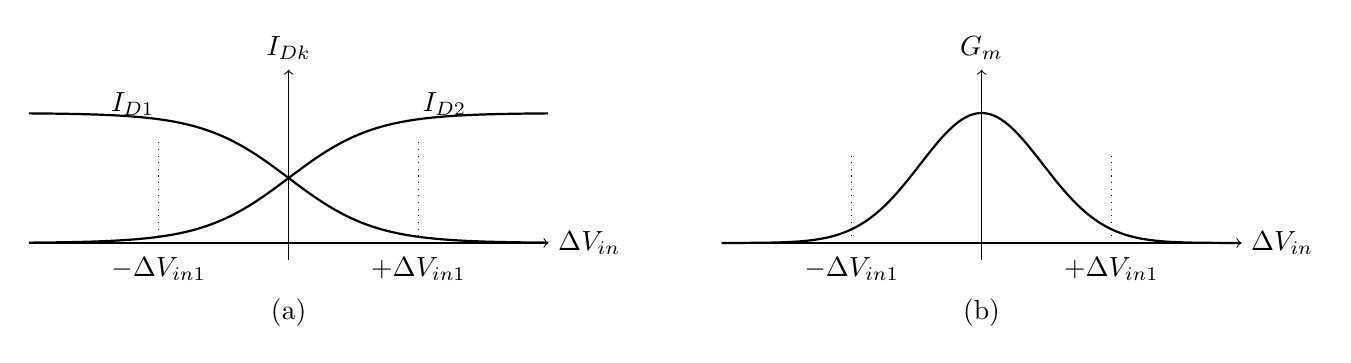
\begin{tikzpicture}[scale=1.1]

% ==== Left Plot - ID1 and ID2 ====
\begin{scope}[xshift=-4cm]

\draw[->] (-3,0) -- (3,0) node[right] {$\Delta V_{in}$};
\draw[->] (0,-0.2) -- (0,2) node[above] {$I_{Dk}$};

% Currents - ID1 and ID2
\draw[thick, domain=-3:3, samples=200, smooth]
plot (\x, {1.5/(1+exp(2*\x))});
\draw[thick, domain=-3:3, samples=200, smooth]
plot (\x, {1.5/(1+exp(-2*\x))});

% Labels
\node at (-1.8,1.6) {$I_{D1}$};
\node at (1.8,1.6) {$I_{D2}$};

% Vertical dashed lines
\draw[dotted] (-1.5,0) -- (-1.5,1.2);
\draw[dotted] (1.5,0) -- (1.5,1.2);
\node at (-1.5,-0.3) {$-\Delta V_{in1}$};
\node at (1.5,-0.3) {$+\Delta V_{in1}$};

% (a) label
\node at (0,-0.8) {(a)};
\end{scope}

% ==== Right Plot - Gm ====
\begin{scope}[xshift=4cm]
% Axes
\draw[->] (-3,0) -- (3,0) node[right] {$\Delta V_{in}$};
\draw[->] (0,-0.2) -- (0,2) node[above] {$G_m$};

% Gm plot
\draw[thick, domain=-3:3, samples=200, smooth]
plot (\x, {1.5*exp(-(\x)^2)});

% Vertical dashed lines
\draw[dotted] (-1.5,0) -- (-1.5,1.0);
\draw[dotted] (1.5,0) -- (1.5,1.0);
\node at (-1.5,-0.3) {$-\Delta V_{in1}$};
\node at (1.5,-0.3) {$+\Delta V_{in1}$};

% (b) label
\node at (0,-0.8) {(b)};
\end{scope}

\end{tikzpicture}
\caption{(a) Plot of Current vs. Differential Input Voltage, (b) Plot of Transconductance}
\end{figure}

\clearpage

\cite{aboushady2016}

\cite{dynapar2025}

\cite{razaviDifferentialPair}


\newpage

\section{Single-ended vs Differential Input Comparison Plot}
\vspace*{2cm}
\begin{figure}[H]
    \centering
    \includegraphics[width=0.95\linewidth]{Chapter_6/Lab-06-LTSpice-Plot.png}
    \caption{In-Phase vs Out-of-Phase Plots of Simulated V(vo)}
    \label{Ch6_fig:4}
\end{figure}

\section{Python Code Listings}

The Python code for differential pair analysis can be found in the Appendix (\cref{lst:Ch6:List1}).

\section{Conclusion}
The lab successfully demonstrated the behavior and advantages of a MOS differential pair, specifically highlighting its performance using the ALD1105 MOSFET array. Through both theoretical analysis and practical implementation, the lab emphasized the superiority of differential signaling over single-ended signaling in terms of noise rejection and signal integrity. The measured DC operating points closely matched simulation predictions, validating the circuit’s proper biasing and symmetrical configuration.

AC analysis further confirmed the benefits of differential operation. The differential gain was significantly higher and more stable, while the common-mode gain was drastically reduced compared to the single-ended configuration. This led to a much higher common-mode rejection ratio (CMRR), both in simulation and measurement, for the differential output. The measured CMRR increased from $21.7$ dB (single-ended) to $48.3$ dB (differential), demonstrating the effectiveness of the differential pair in suppressing common-mode noise.

Theoretical derivations, supported by LTSpice simulations, aligned with experimental results, strengthening the understanding of current steering mechanisms and transconductance behavior in MOS differential amplifiers. In summary, the lab clearly illustrated the functional and practical benefits of differential signaling in analog circuit design, particularly in enhancing noise immunity and ensuring signal fidelity in mixed-signal environments.

\clearpage
\printbibliography[heading=subbibliography]